% appears to be orhapned
The baseline design for the online data handling system is shown schematically in Fig.\ref{fig:topology}.  This design leverages the technology of the Fermilab File Transfer Service (F-FTS) running in two positions within the CERN computing environment.


\begin{figure}[h]
  \centering
  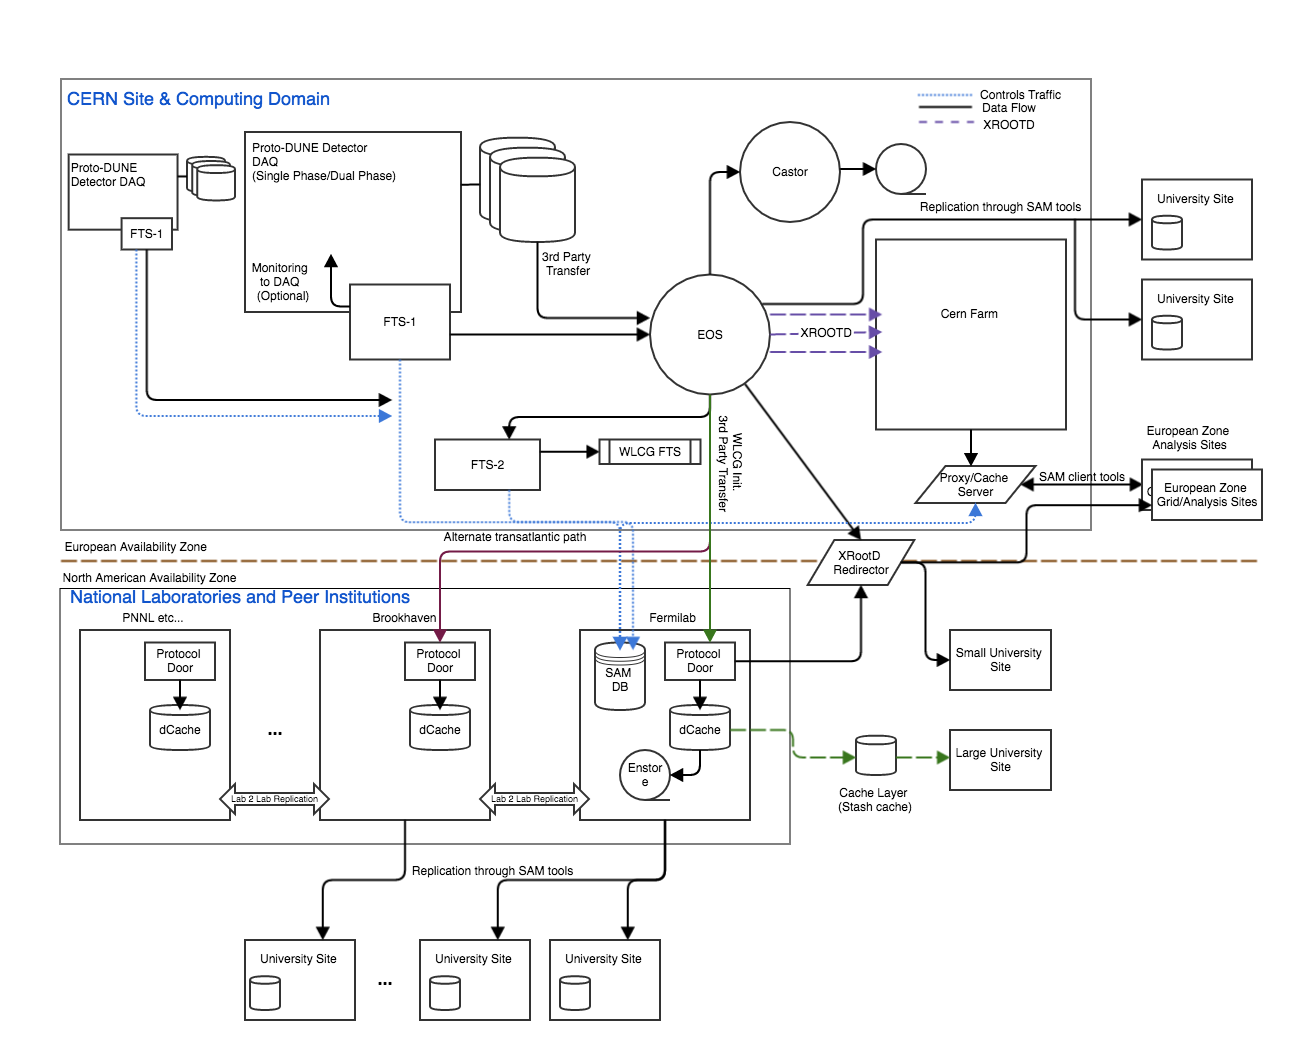
\includegraphics[width=1.0\textwidth]{protDune-datahandling-topology.png}
  \caption{Systems}
  \label{fig:topology}
\end{figure}

A primary F-FTS is homed within the protoDUNE DAQ domain for each of the detector setups (single phase or dual phase readout detectors) and is configured to run on a system which is able to access the DAQ’s buffer disks either through a POSIX filesystem or a protocol layer (e.g. XROOTD, gridFTP or others).  The primary FTS system is configured on this system to look at one or more input directories or storage locations, commonly referred to as a “dropboxes”.  The FTS daemon performs periodic scans of the configured dropboxes.  The system will operate asynchronously and independently of the protoDUNE DAQ systems.  When the protoDUNE DAQ has produced a file that it wishes to have passed off to the storage system, it will “move” (perform a filesystem/storage system atomic move operation or the equivalent) the file to the dropbox location. When a new file is located within one of the dropboxes, the system will initiate the file registration and transfer operations.


In the protoDUNE model, the primary FTS will initiate a copy operation from the online disk buffer farms into the EOS storage system.  The system will use the 3rd party copy support that is provided by the XROOTD protocol to allow for optimized transfers into EOS.  Upon completion of the initial copy into EOS, the FTS will initiate a “chained” copy (a copy that is dependent on the initial copy into EOS) of the data from EOS to the Castor archive system.  The FTS system will register each file’s metadata records (containing both basic and physics metadata, defined below)  in the SAM data handling system.  Upon completion of the replication of the data to Castor, the FTS will enter a monitoring/polling state of its operations to determine when the file has been successfully written to the archival media.
The primary FTS will handle the “cleanup” of its input dropbox.  The FTS performs configurable periodic cleanup passes through its current file sets.  The baseline cleanup logic is shown in Fig. X.  This cleanup process ensures that all files are successfully transferred and archived before they are deleted and provides an “age” criterion on files so that files can be retained within the DAQ environment for a period of time.  This allows operations like online/nearline processing or log files to be examined within the DAQ environment after the actual transfers to archival storage have completed.


The secondary FTS service runs outside of the detector DAQ domains, but within the CERN computing sphere.  This FTS system is configured to monitor as its input dropboxes, the EOS locations that the primary DAQ-FTS systems are using as output endpoints.  The system operates in the same manner as the primary FTS, scanning for new file and then initiating copy requests of the data to a set of one or more destination endpoints.  This FTS system will initiate the copy request between the European availability zone, and the North American availability zone.  At least one of the endpoint destinations for this service will be the FNAL-based dCache/Enstore system, where a second archival copy of the data will be recorded.  Additional copies across the availability zones can be configured based on available resources and available transatlantic bandwidth (e.g. direct transfer from CERN to BNL’s dCache or to PNNL’s storage facilities).  To perform the transfers, the F-FTS will interface with the WLCG FTS (as a supported transfer protocol) to schedule the actual transfer between the storage elements.  